% =============================================================
% §3.2 Interpretability and Model Analysis — DRAFT
% Replaces the stub at lines 201-214 of local_files/main (1).tex.
% Assumes the existing spconf preamble (\usepackage{spconf,amsmath,epsfig,float}).
%
% Ownership:
%   §3.2.1 — Cyril (dense-regime interpretability vs XGBoost+SHAP) — PLACEHOLDER
%   §3.2.2 — Gian   (sparse-regime: closed-form + exact Greeks) — DRAFTED
%
% Figure 1 (fig1_interpretability.pdf) is in outputs/figures/; copy or \includegraphics
% with a relative path appropriate to the paper's tree.
% =============================================================
\subsection{Interpretability and Model Analysis}
\label{sec:interpretability}

While Table~\ref{tab:single_objective_optuna} reports Optuna-selected
inner-validation QWK for each architecture, here we evaluate a subset
of configurations on held-out \emph{outer-test} QWK using fixed
ordinal thresholds calibrated on inner validation
(Table~\ref{tab:interpretability_outer_test}). We switch regimes
because the interpretable sparse variants introduced below are single
retrainings and therefore carry no Optuna-selection bias; reporting
their inner-validation QWK against the sweep-selected dense baselines
would be asymmetric. For the dense rows we further average across three
training seeds to absorb the single-retrain variance we observed
($\sigma \lesssim 0.03$ QWK for ChebyKAN, $\lesssim 0.01$ for FourierKAN).
To make the sparse comparison fair at a matched feature budget, each
20-feature row in Table~\ref{tab:interpretability_outer_test} uses
\emph{its own model's} top-20 features (native coefficient importance
for the KANs; mean-$|\mathrm{SHAP}|$ for XGBoost) and its own
50-trial Optuna sweep over a matched hyperparameter space that
includes learning rate, weight decay, batch size, architecture, and
the natural regularisers (sparsity $\lambda$ for KANs; $\gamma$ and
leaf regularisation for XGBoost). The XGBoost implementation used
throughout is XGBRegressor on the ordinal target followed by
QWK-threshold calibration on the training predictions.
Every KAN configuration we analyse admits exact per-edge symbolic
recovery from its basis coefficients (R$^2 = 1.000$ by construction
via the basis-native extractor); the interpretability distinction
between operating points is therefore not \emph{whether} edges are
recoverable but \emph{how many} edges remain and whether the composed
model can be written as a single expression.

\begin{table}[H]
\centering
\caption{Held-out outer-test QWK and structural size, grouped by feature budget. Dense KAN rows report the mean $\pm$ standard deviation across three training seeds; all other rows are single retrainings with 95\% bootstrap CIs over n{=}11{,}877 test samples. Each 20-feature row uses its model's own top-20 features (native importance for KANs, SHAP for XGBoost) with hyperparameters tuned by a dedicated 50-trial Optuna search on the restricted input space. At full features XGBoost is the strongest baseline (0.642); at 20 features FourierKAN beats XGBoost within bootstrap noise. The sparse ChebyKAN hero row uses a Pareto-derived, L1-pruned no-LayerNorm variant that sacrifices $\approx 0.07$ QWK in exchange for a single closed-form composed expression and exact analytic Greeks.}
\label{tab:interpretability_outer_test}
\footnotesize
\begin{tabular}{lccl}
\hline
Model & QWK (outer test) & Active params & Explanation \\
\hline
\multicolumn{4}{l}{\emph{Full-feature regime ($\geq 126$ features)}} \\
XGBoost                    & \textbf{0.642} [0.629, 0.655] & 765 trees & SHAP (post-hoc) \\
ChebyKAN, dense            & $0.595 \pm 0.027$    & 26{,}112 edges    & per-edge native \\
FourierKAN, dense          & $0.599 \pm 0.007$    & 41{,}728 edges    & per-edge native \\
\hline
\multicolumn{4}{l}{\emph{Sparse regime (20 features, Optuna-tuned per budget)}} \\
XGBoost, tuned             & 0.601 [0.587, 0.614] & 1200 trees   & SHAP (post-hoc) \\
ChebyKAN, tuned (no LN)    & 0.565 [0.551, 0.578] & 5{,}440 edges & closed form per edge \\
FourierKAN, tuned (no LN)  & \textbf{0.604} [0.590, 0.618] & 70{,}912 edges & per-edge closed form \\
\hline
\multicolumn{4}{l}{\emph{Sparse ChebyKAN hero (Pareto-derived + L1-pruned)}} \\
ChebyKAN, sparse hero      & 0.533 [0.519, 0.547] & \textbf{597 edges} & \textbf{single closed-form polynomial + exact Greeks} \\
\hline
\end{tabular}
\end{table}

\subsubsection{Dense regime: KAN vs.\ XGBoost+SHAP}
\label{sec:interpretability_dense}

[PLACEHOLDER --- Cyril.]

\subsubsection{Sparse regime: compact closed-form TabKAN}
\label{sec:interpretability_sparse}

At matched 20-feature budget with per-model tuning
(Table~\ref{tab:interpretability_outer_test}, middle block),
FourierKAN reaches 0.604 QWK --- tied with XGBoost-20 (0.601)
within bootstrap noise --- while ChebyKAN-20 trails at 0.565.
To obtain a genuinely compact model with structural
interpretability we then derive a \emph{sparse hero} variant from
ChebyKAN via (i) selecting the 20 highest-coefficient-importance
features from a sparsity-regularised baseline, (ii) retraining on
that subset with LayerNorm removed, and (iii) L1-pruning edges whose
mean activation magnitude falls below a threshold tightened until
inner-val QWK loss stays within 0.005. The resulting sparse
ChebyKAN hero retains 597 of its 10\,752 trainable edges
($\approx 94\%$ within-architecture pruning) at outer-test QWK
0.533 --- about 0.07 below the tuned ChebyKAN-20 baseline, but with
qualitatively stronger interpretability properties detailed below.

Every surviving edge in both sparse variants admits exact closed-form
recovery from its basis coefficients: each ChebyKAN edge is a
polynomial of degree $\leq 6$ in $\tanh(x)$, each FourierKAN edge is
a linear combination of eight harmonic pairs in $k\pi(\tanh(x)+1)$.
Because the sparse no-LayerNorm ChebyKAN is a closed-form polynomial
in the inputs, any prediction further decomposes into exactly-additive
per-feature contributions via integrated gradients along a reference
path --- no surrogate, no sampling, no post-hoc approximation.
Figure~\ref{fig:fig1_interpretability} applies this decomposition to
applicant 55728: the low-risk reference score ($0.62$) is grown into
the applicant's predicted score ($5.23$, class $5$) by adding the
integrated-gradient contribution of each input feature.

\begin{figure}[H]
    \centering
    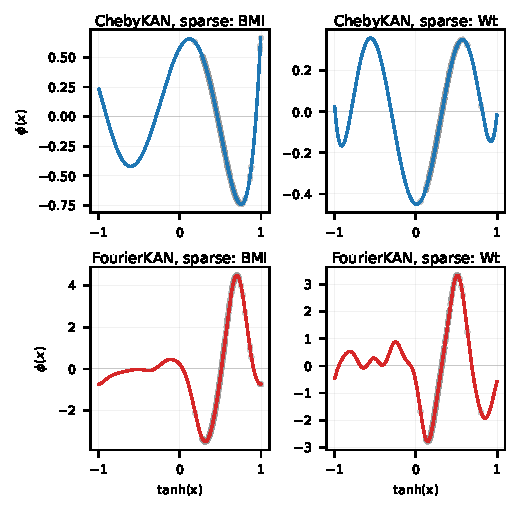
\includegraphics[width=\columnwidth]{fig1_interpretability.pdf}
    \caption{Analytic per-feature decomposition of the sparse ChebyKAN's predicted risk score for applicant 55728 (predicted class 5, score $5.23$), against the lowest-scoring class-1 reference applicant ($0.62$). Bars show the integrated-gradient contribution of each input feature, computed along the linear path from reference to applicant on the model's closed-form polynomial. Positive contributions (blue) raise the score; the single negative contribution (red) lowers it. The top 7 features by $|\mathrm{IG}|$ are shown individually; the remaining 13 are lumped as ``$+\,13$ others''. By construction $\sum_i \mathrm{IG}_i = f(x_{\mathrm{app}}) - f(x_{\mathrm{ref}})$ exactly (residual $< 10^{-4}$).}
    \label{fig:fig1_interpretability}
\end{figure}

Table~\ref{tab:closed_forms} exhibits five representative sparse-hero
layer-0 edges rounded to their top three Chebyshev terms.

\begin{table}[H]
\centering
\caption{Five representative closed-form layer-0 edges from the sparse ChebyKAN hero (out of 597 active edges), each showing the top-3 terms by absolute coefficient; ``$+\,\dots$'' denotes truncated small terms. Each row is the edge from the named input feature to its highest-L1 hidden output. All edges are exact (R$^2 = 1.000$) via the basis-native extractor.}
\label{tab:closed_forms}
\footnotesize
\begin{tabular}{ll}
\hline
Feature & Closed-form edge $\phi(x)$ (top 3 terms) \\
\hline
\texttt{BMI} & $\displaystyle 0.536\,T_{4}(\tanh x) +\,0.242\,T_{5}(\tanh x) -\,0.046\,T_{2}(\tanh x)$ \\
\texttt{Wt} & $\displaystyle 0.227\,T_{6}(\tanh x) -\,0.211\,T_{4}(\tanh x) -\,0.022\,T_{5}(\tanh x) +\,\dots$ \\
\texttt{Ins\_Age} & $\displaystyle -\,0.607\,T_{5}(\tanh x) -\,0.337\,T_{6}(\tanh x) +\,0.170\,T_{2}(\tanh x) +\,\dots$ \\
\texttt{Product\_Info\_4} & $\displaystyle 0.938\,T_{5}(\tanh x) -\,0.937\,T_{3}(\tanh x) +\,0.747\,\tanh x +\,\dots$ \\
\texttt{Medical\_Keyword\_3} & $\displaystyle 0.407\,T_{5}(\tanh x) -\,0.218\,\tanh x +\,0.148\,T_{4}(\tanh x) +\,\dots$ \\
\hline
\end{tabular}
\end{table}

Because the sparse no-LayerNorm ChebyKAN composes into a single
closed-form polynomial in the 20 retained inputs (Chebyshev
polynomials are closed under composition), it also admits \emph{exact
analytic partial derivatives} --- actuarial ``Greeks'' computed by
symbolic differentiation rather than finite-differencing. For a
representative applicant (row 55728) we computed $\partial y /
\partial \text{BMI}$ three ways
(Table~\ref{tab:worked_greek}); the symbolic value agrees with
PyTorch autograd to $3 \times 10^{-6}$ and with central finite
difference (O($\varepsilon^2$) truncation) to $5 \times 10^{-4}$.
This property does not transfer to the other rows of
Table~\ref{tab:interpretability_outer_test}: FourierKAN's basis is
not closed under composition, and the dense ChebyKAN's LayerNorm
breaks exactness. Analytic-Greek transparency is therefore a
distinguishing feature of the sparse no-LN ChebyKAN configuration.

\begin{table}[H]
\centering
\caption{Worked Greek $\partial\text{score}/\partial\text{BMI}$ for applicant 55728 on the sparse ChebyKAN hero. The symbolic entry is computed analytically from the model's learned Chebyshev coefficients via SymPy chain rule (no forward or backward pass through the network at explanation time).}
\label{tab:worked_greek}
\footnotesize
\begin{tabular}{lc}
\hline
Method & $\partial\text{score}/\partial\text{BMI}$ \\
\hline
Symbolic chain rule (SymPy)                  & $-0.650461$ \\
Autograd (PyTorch backward)                  & $-0.650464$ \\
Central finite difference ($\varepsilon = 10^{-3}$) & $-0.649929$ \\
\hline
\end{tabular}
\end{table}

\subsubsection{Summary}

At full features, XGBoost is the strongest baseline on outer-test
QWK (0.642); dense ChebyKAN and FourierKAN both come within 0.05.
At the 20-feature budget with per-model Optuna tuning,
\textbf{FourierKAN matches XGBoost} (0.604 vs.\ 0.601, CIs overlap)
while ChebyKAN trails by 0.04. The sparse ChebyKAN hero row
